% Created 2023-05-24 Wed 20:58
% Intended LaTeX compiler: pdflatex
\documentclass[a4paper,twocolumn]{article}
\usepackage[utf8]{inputenc}
\usepackage[T1]{fontenc}
\usepackage{graphicx}
\usepackage{longtable}
\usepackage{wrapfig}
\usepackage{rotating}
\usepackage[normalem]{ulem}
\usepackage{amsmath}
\usepackage{amssymb}
\usepackage{capt-of}
\usepackage{hyperref}
\usepackage[T1]{fontenc}
\usepackage{tgbonum}
\usepackage{biblatex}
\addbibresource{/home/dp/Documents/Research_paper_SFR/bibl/bibliography/bibliography.bib}
\usepackage{amsmath}
\usepackage{graphicx}
\usepackage{caption}
\usepackage{booktabs}
\usepackage{hyperref}
\let\description\compactdesc
\raggedbottom
\date{\today}
\title{Finding Adel}
\hypersetup{
 pdfauthor={},
 pdftitle={Finding Adel},
 pdfkeywords={},
 pdfsubject={},
 pdfcreator={Emacs 28.2 (Org mode 9.6.1)}, 
 pdflang={English}}
\begin{document}

\maketitle


\section{Delayed-\(\tau\) model}
\label{sec:orgfa1060d}

According to P. Kroupa et al. 2020\autocite{kroupaConstraintsStarFormation2020} current star formation rates of galaxies can be described by the 'delayed-\(\tau\)' model as


\begin{equation} \label{eq:SFR}
SFR_{0,del}=\frac{A_{del}xe^{-x}}{\tau},\text{ where } x=\frac{t_{sf}}{\tau}
\end{equation}

\noindent
where \(\tau\) is the star formation time-scale,  \(t_{sf}\) is the real time of star formation in a given galaxy and \(A_{del}\) a normalization constant.

The average SFR is

\begin{equation}\label{eq:av_SFR-x}
\overline{SFR_{del}}=\frac{A_{del}}{t_{sf}}[1-(1+x)e^{-x}]
\end{equation}
and can also be defined by the present day stellar mass

\begin{equation}\label{eq:av_SFR M*}
    \overline{SFR}=\frac{\zeta M_*}{t_{sf}}
\end{equation}
where \(\zeta\) accommodates for mass-loss through stella evolution and \(\zeta\approx 1.3\)

This is a system of 2 equations and 3 variables, since A\textsubscript{del} has never been calculated


\subsection{Constant \(t_{sf}\)}
\label{sec:org8a4d333}
The observed ages of galactic discs are \(t_{sf}\approx 12\) Gyr\autocite{knoxSurveyCoolWhite1999}, so assuming an approximation of \(t_{sf}=12.5\) Gyr, the \(\overline{SFR_{del}}\) can be calcuated, from the equation (\ref{eq:av_SFR M*}).


After that the equation of ratio


\begin{equation} \label{eq:ratio}
    \frac{\overline{SFR_{del}}}{SFR_{0,del}}=\frac{e^x-x-1}{x^2}
\end{equation}

can be solved numerically for \(x\) and using the equations (\Ref{eq:SFR}) and (\Ref{eq:av_SFR-x}) the \(A_{del}\) and \(\tau\) of each galaxy are found.




\begin{center}
\begin{tabular}{lrrr}
 & \(A_{tsf}\) & \(\tau\) & \(x_{tsf}\)\\[0pt]
\hline
count & 578 & 579 & 579\\[0pt]
mean & 2.24715e+12 & 1.08958e+11 & 1.853\\[0pt]
std & 3.93675e+13 & 1.04132e+12 & 1.476\\[0pt]
min & 2.47798e+07 & 1.93205e+09 & 0.001\\[0pt]
25\% & 1.40573e+08 & 4.18098e+09 & 0.565\\[0pt]
50\% & 6.83764e+08 & 7.79265e+09 & 1.604\\[0pt]
75\% & 5.70379e+09 & 2.21327e+10 & 2.99\\[0pt]
max & 9.10088e+14 & 2.23774e+13 & 6.47\\[0pt]
\end{tabular}
\end{center}


\begin{figure}[!htpb]
\centering
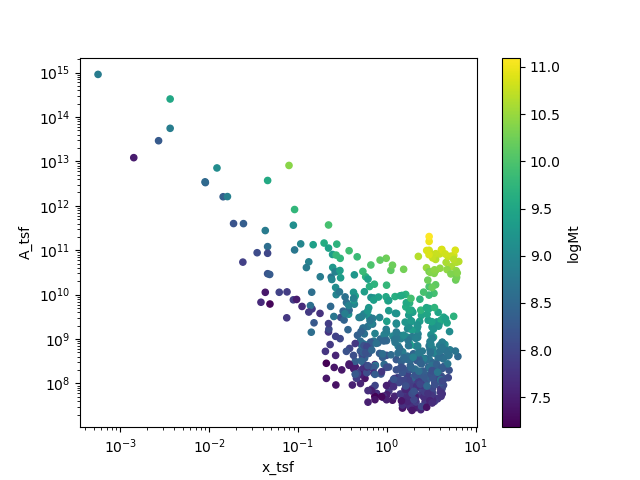
\includegraphics[width=.9\linewidth]{./figs/x-A_tsf.png}
\caption{\label{fig:$A_{del} = f(x)$ for constant t_{sf}}\(A_{del} = f(x)\) for constant t\textsubscript{sf}}
\end{figure}


\begin{figure}[!htpb]
\centering
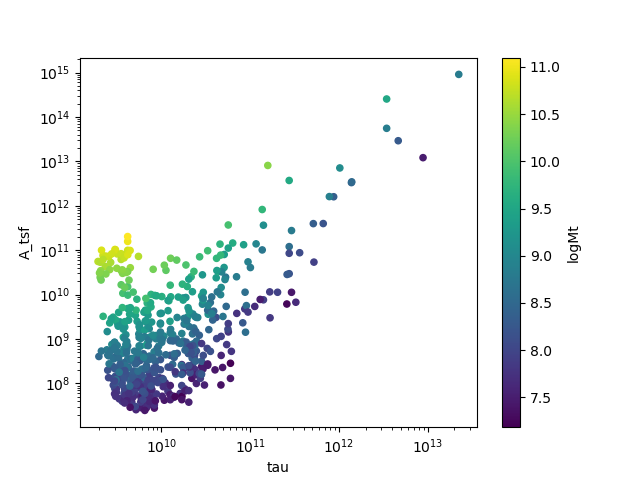
\includegraphics[width=.9\linewidth]{./figs/T-A_tsf.png}
\caption{\label{fig:$A_{del} = f(\tau)$ for constant t_{sf}}\(A_{del} = f(\tau)\) for constant t\textsubscript{sf}}
\end{figure}


\begin{figure}[!htpb]
\centering
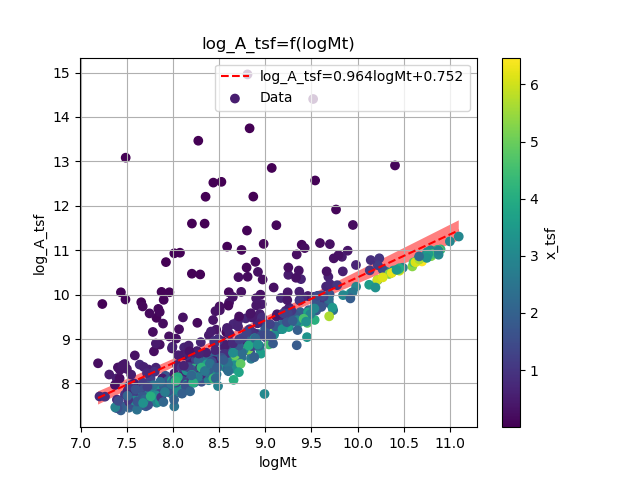
\includegraphics[width=.9\linewidth]{./figs/logMt-log_A_tsf-color_x_tsf.png}
\caption{\label{fig:A_tsf_Mt}Total Mass \(M_t\) - \(A_{del}|_{t_{sf}}\)}
\end{figure}

\begin{equation}\label{eq:logMt-log_A_tsf-color_x_tsf}
\begin{align}
& $log(A_{del}|_t_{sf}) = (9.6(4) \times 10^{-1})\cdot $log(M_t)$ + (8(4) \times 10^{-1}) \\
& \textrm{with correlation } R^2=48\%
\end{align}
\end{equation}
\noindent


\pagebreak
\subsection{Constant \(\tau\)}
\label{sec:org59966a2}


Assuming for an constant \(\tau=3.5\) Gyr, we cannot use the same \(\overline{SFR}\) since it depends on \(t_{sf}\). Using the equations\textasciitilde{}(\Ref{eq:av_SFR M*}) and (\Ref{eq:ratio})

$$
    \frac{\overline{SFR_{del}}}{SFR_{0,del}}=\frac{e^x-x-1}{x^2}\Leftrightarrow \frac{e^x-x-1}{x}=\frac{\zeta M_*}{SFR\cdot\tau}
$$

using this equation \(x\) and \(A_{del}\) can be calculated numerically.


\begin{center}
\begin{tabular}{lrrr}
 & \(A_\tau\) & \(x_\tau\) & \(t_{sf}\)\\[0pt]
\hline
count & 579 & 579 & 579\\[0pt]
mean & 4.58667e+09 & 2.54057 & 8.89201e+09\\[0pt]
std & 1.49896e+10 & 0.956554 & 3.34794e+09\\[0pt]
min & 9.87003e+06 & 0.406787 & 1.42376e+09\\[0pt]
25\% & 6.50497e+07 & 1.87165 & 6.55079e+09\\[0pt]
50\% & 2.36667e+08 & 2.43871 & 8.5355e+09\\[0pt]
75\% & 1.11526e+09 & 3.07972 & 1.0779e+10\\[0pt]
max & 1.0577e+11 & 5.77102 & 2.01986e+10\\[0pt]
\end{tabular}
\end{center}

\begin{figure}[!htpb]
\centering
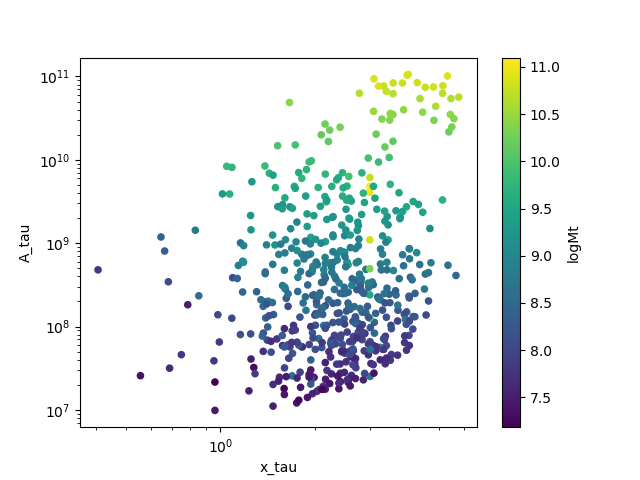
\includegraphics[width=.9\linewidth]{./figs/x-A_tau.png}
\caption{\label{fig:$A_{del} = f(x)$ for constant $\tau$}\(A_{del} = f(x)\) for constant \(\tau\)}
\end{figure}


\begin{figure}[!htpb]
\centering
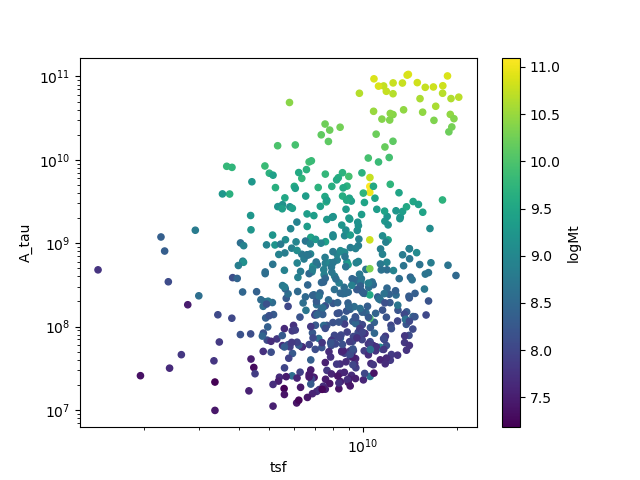
\includegraphics[width=.9\linewidth]{./figs/T-A_tau.png}
\caption{\label{fig:$A_{del} = f(t_{sf})$ for constant $\tau$}\(A_{del} = f(t_{sf})\) for constant \(\tau\)}
\end{figure}

\begin{figure}[!htpb]
\centering
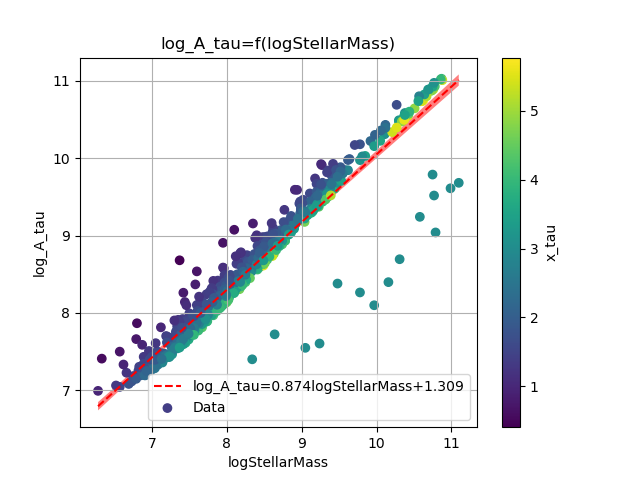
\includegraphics[width=.9\linewidth]{./figs/logStellarMass-log_A_tau-color_x_tau.png}
\caption{\label{fig:A_tau_Mt}Total Mass \(M_t\) - \(A_{del}|_{\tau}\)}
\end{figure}

\begin{equation}\label{eq:logStellarMass-log_A_tau-color_x_tau}
\begin{align}
& $log(A_{del}|_\tau) = (8.74(12) \times 10^{-1})\cdot $log(M_t)$ + (1.31(10) \times 10^{0}) \\
& \textrm{with correlation } R^2=90\%
\end{align}
\end{equation}
\noindent


\pagebreak
\subsection{Comparing the two results}
\label{sec:org531854c}

\subsubsection{Comparing the \(x\)'s}
\label{sec:org8a255b5}


Comparing the two different results for x, we see that the \(x|_\tau\) has a lower \(\sigma\)


\begin{table}[hc]
\centering
\begin{tabular}{lrr}
\toprule
{} &    $x|_\tau$ & $x|_{tsf}$ \\
\midrule
count & 5.79E+02 & 5.79E+02 \\
mean  & 2.54E+00 & 1.85E+00 \\
std   & 9.57E-01 & 1.48E+00 \\
min   & 4.07E-01 & 5.59E-04 \\
25\%   & 1.87E+00 & 5.65E-01 \\
50\%   & 2.44E+00 & 1.60E+00 \\
75\%   & 3.08E+00 & 2.99E+00 \\
max   & 5.77E+00 & 6.47E+00 \\
\bottomrule
\end{tabular}
\end{table}

\begin{figure}[!htpb]
\centering
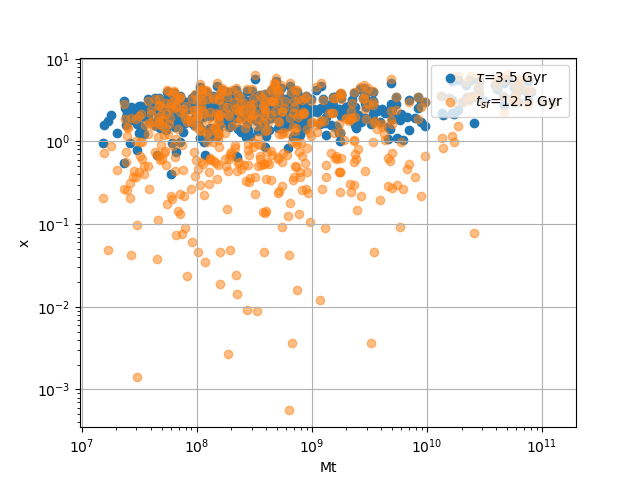
\includegraphics[width=.9\linewidth]{./figs/Comparing_the_x_Mt.png}
\caption{\label{fig:Comparing the two x's, According to their total masses}Comparing the two x's, According to their total masses}
\end{figure}

\begin{figure}[!htpb]
\centering
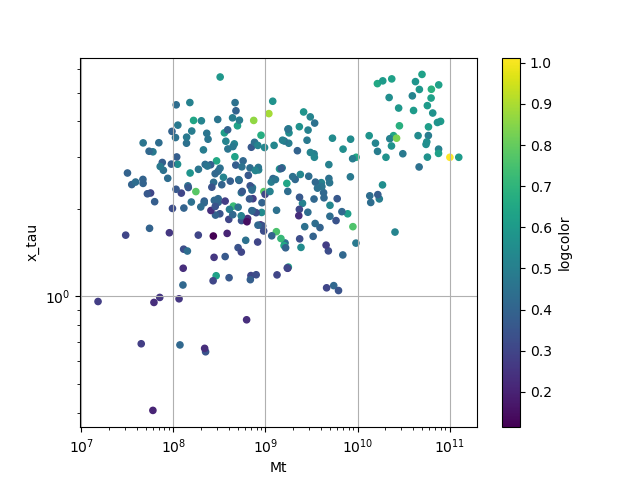
\includegraphics[width=.9\linewidth]{./figs/x_tau-Mt-color.png}
\caption{\label{fig:$x|_\tau=f(M_t)$, with their color index}\(x|_\tau=f(M_t)\), with their color index}
\end{figure}

\begin{figure}[!htpb]
\centering
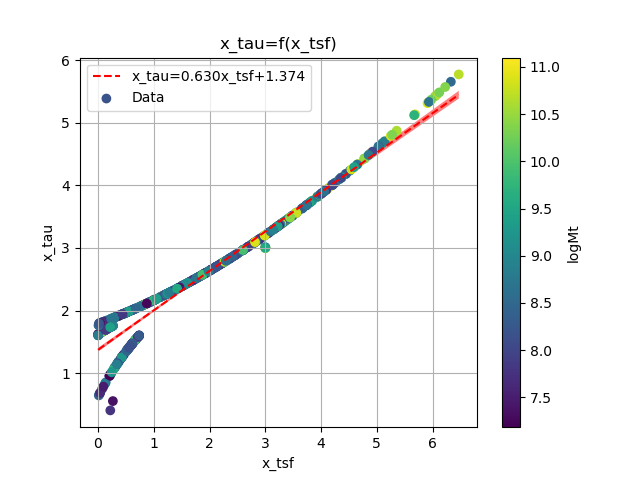
\includegraphics[width=.9\linewidth]{./figs/x_tsf-x_tau-color_logMt.png}
\caption{\label{fig:Comparing the two x, according to their total mass}Comparing the two x, according to their total mass}
\end{figure}

\begin{figure}[!htpb]
\centering
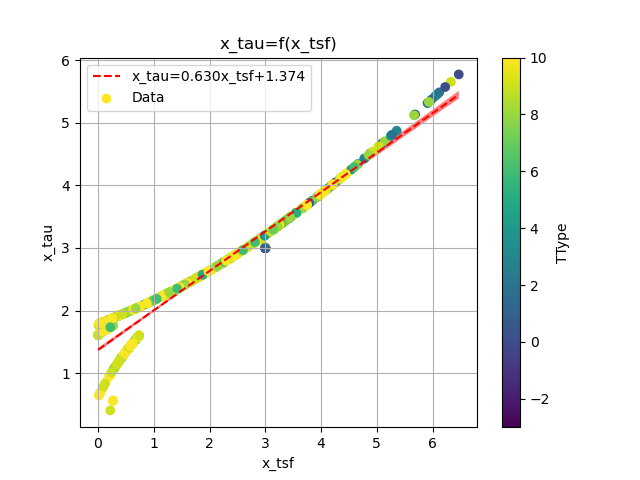
\includegraphics[width=.9\linewidth]{./figs/x_tsf-x_tau-color_TType.png}
\caption{\label{fig:Comparing the two x, according to their type}Comparing the two x, according to their type}
\end{figure}

\begin{figure}[!htpb]
\centering
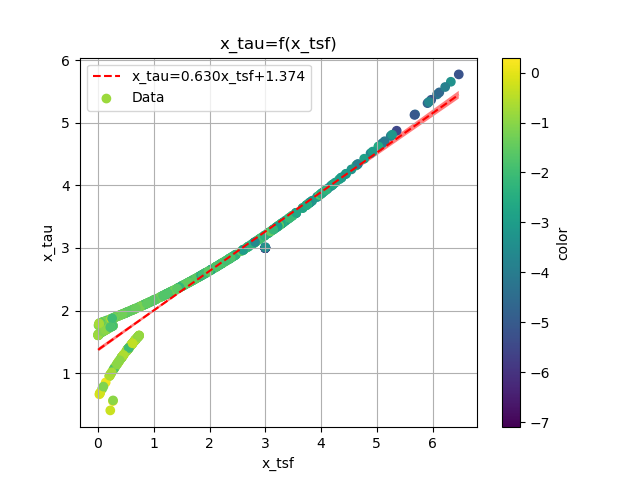
\includegraphics[width=.9\linewidth]{./figs/x_tsf-x_tau-color_color.png}
\caption{\label{fig:Comparing the two x, according to their color index}Comparing the two x, according to their color index}
\end{figure}

The two results are interrelated through the equation:

\begin{equation}\label{eq:x_tsf-x_tau}
\begin{align}
& x|_\tau = (6.30(6) \times 10^{-1})\cdot x|_{tsf} + (1.374(15) \times 10^{0}) \\
& \textrm{with correlation } R^2=94\%
\end{align}
\end{equation}
\noindent

and from the plots the following conclusions can be drawn:

\begin{enumerate}
\item The galaxies with a higher total mass deviate less from the linear fit and are older.
\item The younger galaxies are mainly later types of galaxies
\item For lower x's, the galaxies have a lower color index which indicates that they are younger. So the values are inline with the experimental values.
\end{enumerate}

\subsubsection{Comparing the normalization constants}
\label{sec:org5474350}

\begin{figure}[!htpb]
\centering
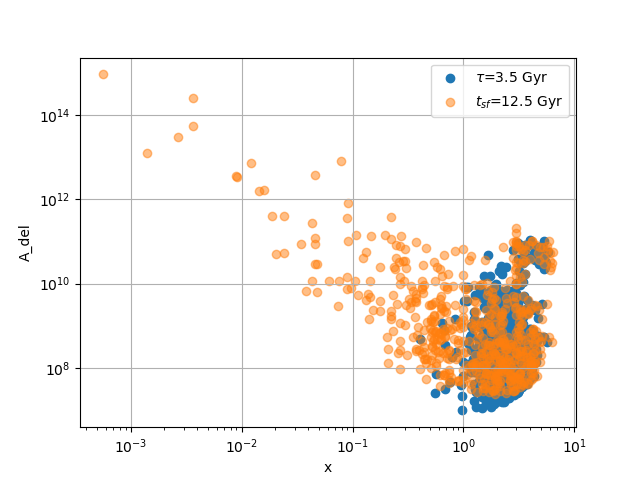
\includegraphics[width=.9\linewidth]{./figs/Comparing_the_A_x.png}
\caption{\label{fig:Comparing the two A_{del}}Comparing the two A\textsubscript{del}}
\end{figure}


\begin{figure}[!htpb]
\centering
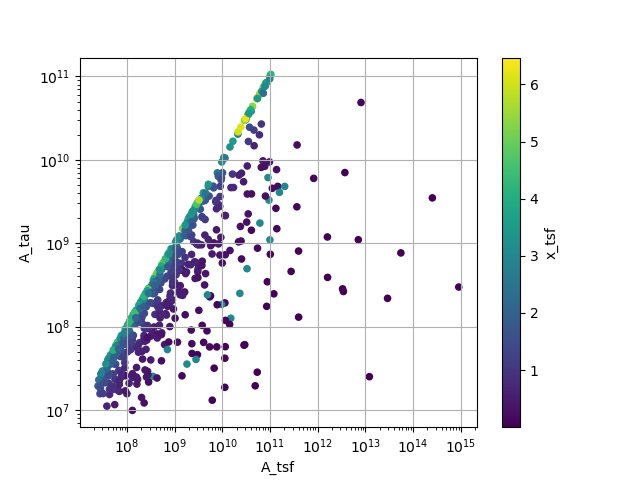
\includegraphics[width=.9\linewidth]{./figs/A_tau-A_tsf_colo_X.png}
\caption{\label{fig:Comparison of the 2 A_{del}s according to their $x$}Comparison of the 2 A\textsubscript{del}s according to their \(x\)}
\end{figure}

\begin{figure}[!htpb]
\centering
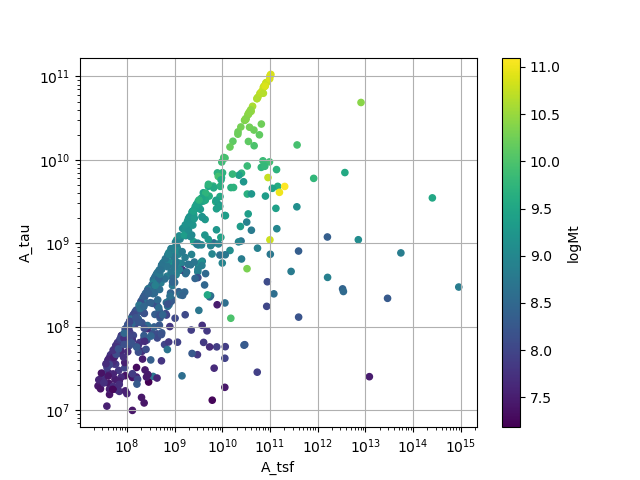
\includegraphics[width=.9\linewidth]{./figs/A_tau-A_tsf_Mt.png}
\caption{\label{fig:Comparison of the 2 A_{del}s according to their total masses}Comparison of the 2 A\textsubscript{del}s according to their total masses}
\end{figure}

For high \(x\) and high masses the two A\textsubscript{del}s have a high correlation. Specifically:
\begin{enumerate}
\item For high \(x\) the \(A_{del}|_{\tau}-A_{del}|_{t_{sf}}\) plot follows a \(y=x\) trend, which means that for older stars and stars with a low star formation timescale \(\tau\), the normalization constant is the same despite the method used to calculate it.
\item The same is true for more massive galaxies, since they deviate less from the \(y=x\) line
\end{enumerate}


\subsection{Int SFR to find the A\textsubscript{del}}
\label{sec:org13c70a8}

If we integrate equation (\ref{eq:SFR}) we get:


\begin{equation}\label{eq:int SFR}
\begin{align}
\int^{t_{sf}}_0 SFR_{del} dt_{sf}&=\int^{t_{sf}}_0 \frac{A_{del}t_{sf}e^{-t_{sf}/\tau}}{\tau^2} dt_{sf}\\
\zeta\cdot M_*&=-A_{del} \frac{{\left(t_{\mathit{sf}} \tau + \tau^{2}\right)} e^{\left(-\frac{t_{\mathit{sf}}}{\tau}\right)}}{\tau^{2}}+A_{del}\\
\zeta\cdot M_*&=-A_{del}\frac{\tau^2(x+1)e^{-x}}{\tau^2}+A_{del}\\
\zeta\cdot M_*& = A_{del}(1-(x+1)e^{-x})\\
A_{del}&=\zeta\cdot M_*\frac{e^x}{e^x-x-1}
\end{align}
\end{equation}

The integral \(\int SFR dt=\) The total mass that is turned into stars. But during the evolution of the stars, the stars spew mass to Interstellar space, so the galaxies lose mass during this process. So the observed Stellar Mass M\textsubscript{*} is smaller than the total mass turned into Stellar Mass.

The constant \(\zeta\) accommodates for this mass-loss and, as discussed earlier, we can assume a conservative value of 1.3 for the galaxies in the LCV.


\begin{figure}[!htpb]
\centering
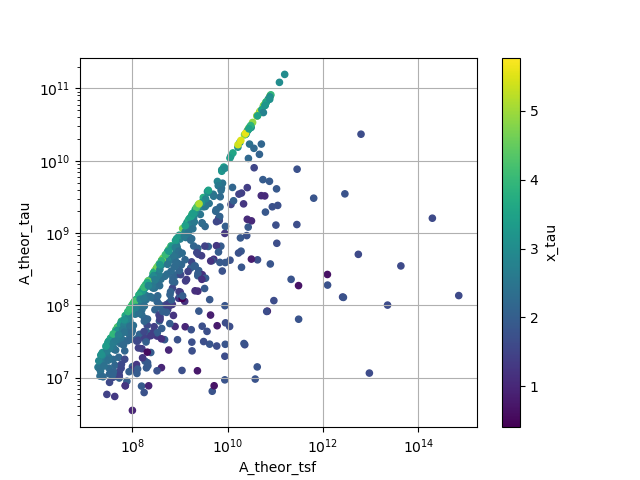
\includegraphics[width=.9\linewidth]{./figs/A_theor_tau-M*.png}
\caption{\label{fig:Comparison of the 2 A_{del}s according to their total masses}Comparison of the 2 A\textsubscript{del}s according to their total masses}
\end{figure}

\begin{figure}[!htpb]
\centering
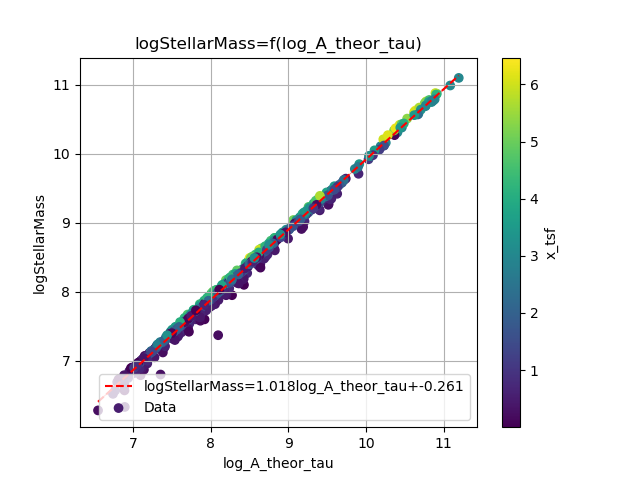
\includegraphics[width=.9\linewidth]{./figs/log_A_theor_tau-logStellarMass-color_x_tsf.png}
\caption{\label{fig:Comparison of the A_del according to their Stellar Mass}Comparison of the A\textsubscript{del} according to their Stellar Mass}
\end{figure}


\begin{figure}[!htpb]
\centering
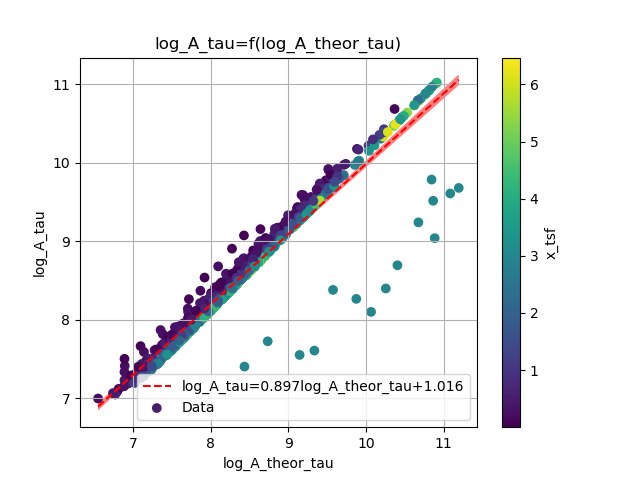
\includegraphics[width=.9\linewidth]{./figs/log_A_theor_tau-log_A_tau-color_x_tsf.png}
\caption{\label{fig:A_theor_A_exp_tau}Comparison of the 2 \$A\textsubscript{del}|\textsubscript{\(\tau\)=const.}\$s (theoretical and experimental)}
\end{figure}

\begin{figure}[!htpb]
\centering
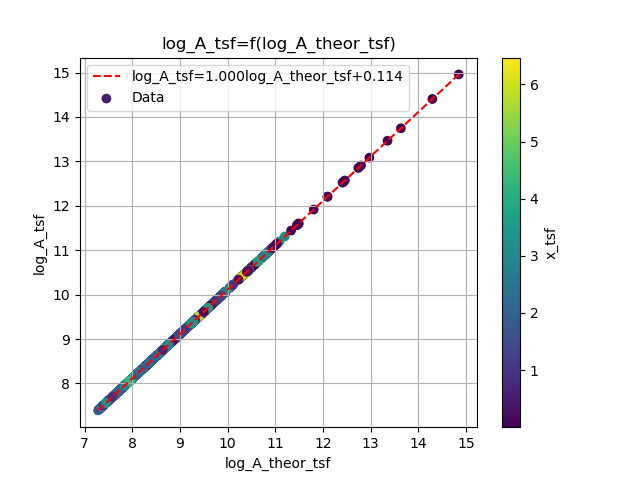
\includegraphics[width=.9\linewidth]{./figs/log_A_theor_tsf-log_A_tsf-color_x_tsf.png}
\caption{\label{fig:A_theor_A_exp_tsf}Comparison of the 2 \$A\textsubscript{del}|\textsubscript{tsf=const.}\$s (theoretical and experimental)}
\end{figure}


From the plots we get correlations of \(R^2 = 91\%\)  and \(A_{tsf} = (8.97(12) \times 10^{-1})\cdot A_{tsf\,theor} + (1.02(10) \times 10^{0})\)  so the theoretical values fit the experimental.

From the equations (\ref{eq:SFR}), (\ref{eq:av_SFR-x}) and (\ref{eq:int SFR}), the \(SFR_{0,del}\) and the \(\overline{SFR_{del}}\) are given by the equations:

\begin{equation} \label{eq:SFR final}
\begin{align}
SFR_{0,del}&=\zeta M_*\frac{e^x}{e^x-x-1}\frac{xe^{-x}}{\tau}\\
          &=\zeta M_*\frac{x}{\tau(e^x-x-1)}
\end{align}
\end{equation}


\begin{equation}\label{eq:av_SFR-x final}
\begin{align}
\overline{SFR_{del}}&=\zeta M_*\frac{e^x}{e^x-x-1}\frac{1}{t_{sf}}[1-(1+x)e^{-x}]\\
                   &=\zeta M_*\frac{e^x}{e^x-x-1}\frac{1}{t_{sf}}\frac{e^x-x-1}{e^x}\\
                   &=\zeta \frac{M_*}{t_{sf}}
\end{align}
\end{equation}

The new \(\overline{SFR_{del}}\) is the same with the \(\overline{SFR}\) of the equation (\ref{eq:av_SFR M*}).


\begin{figure}[!htpb]
\centering
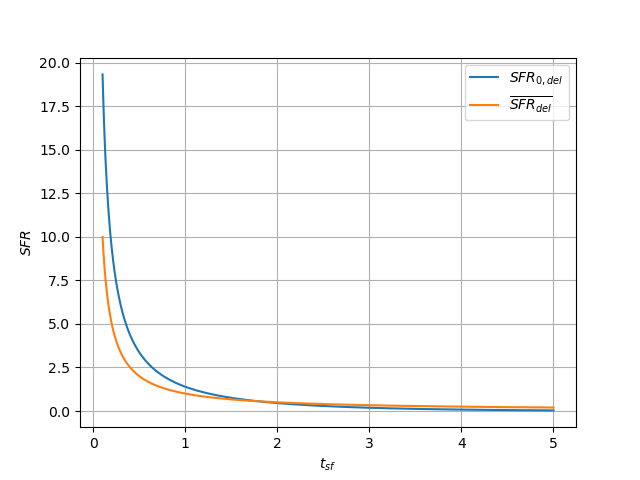
\includegraphics[width=.9\linewidth]{./figs/SFR_avSFR.png}
\caption{\label{fig:The $SFR_{0,del}$ and $\overline{SFR_{del}}$ for constant $\tau=1$ and $\zeta M_*=1$}The \(SFR_{0,del}\) and \(\overline{SFR_{del}}\) for constant \(\tau=1\) and \(\zeta M_*=1\)}
\end{figure}

\pagebreak

\subsection{Calculating the \(t_{sf}\) and \(\tau\) for each galaxy}
\label{sec:org1230772}

Having found an expression for the \(A_{del}\), we have eliminated on out of the 3 variables and now the \(t_{sf}\) and \(\tau\) of each galaxy can be calcuated.



\subsubsection{Method 1}
\label{sec:org9e16912}
\begin{figure}[!htpb]
\centering
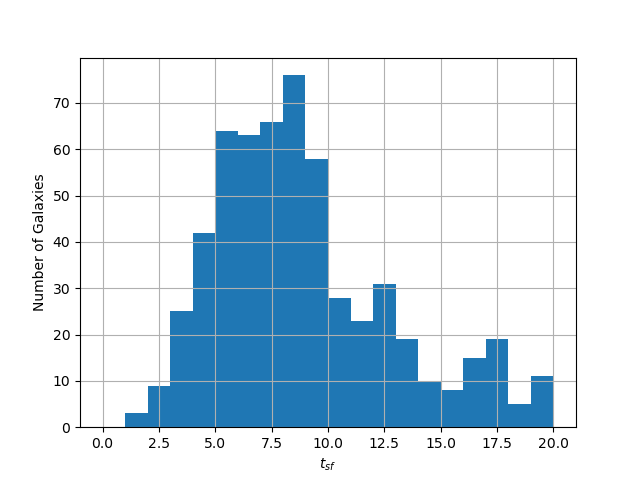
\includegraphics[width=.9\linewidth]{./figs/tsf-hist.png}
\caption{\label{fig:Histogram of t_{sf} from 0 to 20 Gyr}Histogram of t\textsubscript{sf} from 0 to 20 Gyr}
\end{figure}


\begin{center}
\begin{tabular}{lrrr}
 & \(t_{sf}\) Gyr & \(\tau\) Gyr & x\\[0pt]
\hline
count & 579 & 579 & 579\\[0pt]
mean & 9.047 & 3.429 & 2.548\\[0pt]
std & 4.637 & 1.197 & 0.849\\[0pt]
min & 1.307 & 1.262 & 0.642\\[0pt]
25\% & 6.066 & 2.954 & 1.99\\[0pt]
50\% & 8.238 & 3.297 & 2.467\\[0pt]
75\% & 11.007 & 3.691 & 2.962\\[0pt]
max & 62.635 & 27.605 & 9.487\\[0pt]
\end{tabular}
\end{center}


\subsubsection{Method 2}
\label{sec:org21a3006}
\begin{center}
\begin{tabular}{lrrr}
 & \(t_{sf,2}\) Gyr & \(\tau_2\) Gyr & x\\[0pt]
\hline
count & 579 & 579 & 579\\[0pt]
mean & 27.005 & 9.848 & 2.743\\[0pt]
std & 112.566 & 41.066 & 0\\[0pt]
min & 0.523 & 0.191 & 2.738\\[0pt]
25\% & 4.329 & 1.578 & 2.743\\[0pt]
50\% & 7.345 & 2.678 & 2.743\\[0pt]
75\% & 14.071 & 5.13 & 2.743\\[0pt]
max & 1439.37 & 525.624 & 2.743\\[0pt]
\end{tabular}
\end{center}

\begin{figure}[!htpb]
\centering
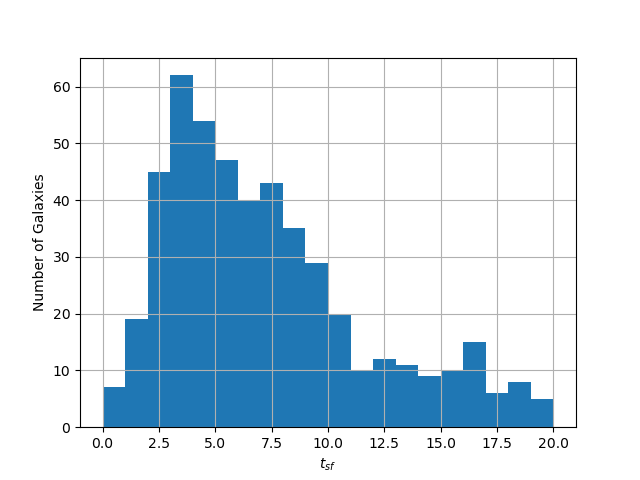
\includegraphics[width=.9\linewidth]{./figs/tsf2-hist.png}
\caption{\label{fig:Histogram of t_{sf} from 0 to 20 Gyr}Histogram of t\textsubscript{sf} from 0 to 20 Gyr}
\end{figure}


\begin{figure}[!htpb]
\centering
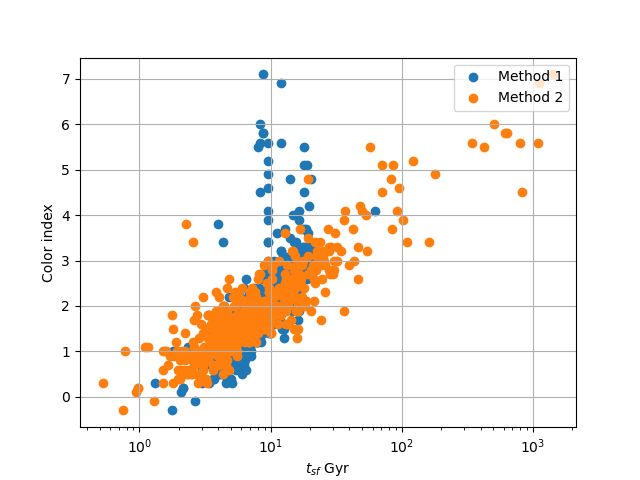
\includegraphics[width=.9\linewidth]{./figs/tsf_tsf2.png}
\caption{\label{fig:Comparing the two $t_{sf}$}Comparing the two \(t_{sf}\)}
\end{figure}



\subsubsection{[?]}
\label{sec:org84e38fd}
\begin{itemize}
\item Can we calculate/observe \(\zeta\)?
\begin{itemize}
\item If not: for galaxies with extreme star-bursting and low-metallicity galaxies \(\zeta=2-3\). Can we find those galaxies and approximate the \(\zeta\)?
\end{itemize}
\item Why couldn't we use (\ref{eq:av_SFR M*}) to calculate \(A_{del}\)
\item While in the second method we see a better correlation between the age of the galaxy and the color index, we must have an older universe
\end{itemize}



\pagebreak
\printbibliography
\end{document}